%%% Humphrey, Gloss, et al.
%%% ESM for,
%%% Heritable plant phenotypes track light and herbivory levels at fine spatial scales
%%% Citation: Humphrey, P.T., Gloss, A.D., Frazier, J. et al. Oecologia (2018). https://doi.org/10.1007/s00442-018-4116-4
%%% Last edited: 11 Mar 2018 by PTH


\documentclass[11pt, oneside]{amsart}
\usepackage[bottom=1in]{geometry}
\usepackage[parfill]{parskip}
\usepackage{graphicx}
\usepackage{amssymb}
\usepackage{epstopdf}
\usepackage{tabu}
\usepackage{booktabs}
\usepackage{etoolbox}


\pagestyle{plain}

\DeclareGraphicsRule{.tif}{png}{.png}{`convert #1 `dirname #1`/`basename #1 .tif`.png}
\DeclareMathOperator{\logit}{logit}
\newcommand{\lib}[1]{\texttt{#1}}
\renewcommand{\thetable}{S\arabic{table}}
\renewcommand{\thefigure}{S\arabic{figure}}
\newcommand\tab[1][0.75cm]{\hspace*{#1}}

%%%%%%%%%%%%% MACRO EDITS TO AMSART ToC %%%%%%%%%%%%%
% Modifications to amsart ToC-related macros...
% i.e., makes pretty ToC for AMSART doc template.
\makeatletter
\let\old@tocline\@tocline
\let\section@tocline\@tocline
% Insert a dotted ToC-line for \subsection and \subsubsection only
\newcommand{\subsection@dotsep}{4.5}
\newcommand{\subsubsection@dotsep}{4.5}
\patchcmd{\@tocline}
  {\hfil}
  {\nobreak
     \leaders\hbox{$\m@th
        \mkern \subsection@dotsep mu\hbox{.}\mkern \subsection@dotsep mu$}\hfill
     \nobreak}{}{}
\let\subsection@tocline\@tocline
\let\@tocline\old@tocline

\patchcmd{\@tocline}
  {\hfil}
  {\nobreak
     \leaders\hbox{$\m@th
        \mkern \subsubsection@dotsep mu\hbox{.}\mkern \subsubsection@dotsep mu$}\hfill
     \nobreak}{}{}
\let\subsubsection@tocline\@tocline
\let\@tocline\old@tocline

\let\old@l@subsection\l@subsection
\let\old@l@subsubsection\l@subsubsection

\def\@tocwriteb#1#2#3{%
  \begingroup
    \@xp\def\csname #2@tocline\endcsname##1##2##3##4##5##6{%
      \ifnum##1>\c@tocdepth
      \else \sbox\z@{##5\let\indentlabel\@tochangmeasure##6}\fi}%
    \csname l@#2\endcsname{#1{\csname#2name\endcsname}{\@secnumber}{}}%
  \endgroup
  \addcontentsline{toc}{#2}%
    {\protect#1{\csname#2name\endcsname}{\@secnumber}{#3}}}%

% Handle section-specific indentation and number width of ToC-related entries
\newlength{\@tocsectionindent}
\newlength{\@tocsubsectionindent}
\newlength{\@tocsubsubsectionindent}
\newlength{\@tocsectionnumwidth}
\newlength{\@tocsubsectionnumwidth}
\newlength{\@tocsubsubsectionnumwidth}
\newcommand{\settocsectionnumwidth}[1]{\setlength{\@tocsectionnumwidth}{#1}}
\newcommand{\settocsubsectionnumwidth}[1]{\setlength{\@tocsubsectionnumwidth}{#1}}
\newcommand{\settocsubsubsectionnumwidth}[1]{\setlength{\@tocsubsubsectionnumwidth}{#1}}
\newcommand{\settocsectionindent}[1]{\setlength{\@tocsectionindent}{#1}}
\newcommand{\settocsubsectionindent}[1]{\setlength{\@tocsubsectionindent}{#1}}
\newcommand{\settocsubsubsectionindent}[1]{\setlength{\@tocsubsubsectionindent}{#1}}

% Handle section-specific formatting and vertical skip of ToC-related entries
% \@tocline{<level>}{<vspace>}{<indent>}{<numberwidth>}{<extra>}{<text>}{<pagenum>}
\renewcommand{\l@section}{\section@tocline{1}{\@tocsectionvskip}{\@tocsectionindent}{}{\@tocsectionformat}}%
\renewcommand{\l@subsection}{\subsection@tocline{1}{\@tocsubsectionvskip}{\@tocsubsectionindent}{}{\@tocsubsectionformat}}%
\renewcommand{\l@subsubsection}{\subsubsection@tocline{1}{\@tocsubsubsectionvskip}{\@tocsubsubsectionindent}{}{\@tocsubsubsectionformat}}%
\newcommand{\@tocsectionformat}{}
\newcommand{\@tocsubsectionformat}{}
\newcommand{\@tocsubsubsectionformat}{}
\expandafter\def\csname toc@1format\endcsname{\@tocsectionformat}
\expandafter\def\csname toc@2format\endcsname{\@tocsubsectionformat}
\expandafter\def\csname toc@3format\endcsname{\@tocsubsubsectionformat}
\newcommand{\settocsectionformat}[1]{\renewcommand{\@tocsectionformat}{#1}}
\newcommand{\settocsubsectionformat}[1]{\renewcommand{\@tocsubsectionformat}{#1}}
\newcommand{\settocsubsubsectionformat}[1]{\renewcommand{\@tocsubsubsectionformat}{#1}}
\newlength{\@tocsectionvskip}
\newcommand{\settocsectionvskip}[1]{\setlength{\@tocsectionvskip}{#1}}
\newlength{\@tocsubsectionvskip}
\newcommand{\settocsubsectionvskip}[1]{\setlength{\@tocsubsectionvskip}{#1}}
\newlength{\@tocsubsubsectionvskip}
\newcommand{\settocsubsubsectionvskip}[1]{\setlength{\@tocsubsubsectionvskip}{#1}}

% Adjust section-specific ToC-related macros to have a fixed-width numbering framework
\patchcmd{\tocsection}{\indentlabel}{\makebox[\@tocsectionnumwidth][l]}{}{}
\patchcmd{\tocsubsection}{\indentlabel}{\makebox[\@tocsubsectionnumwidth][l]}{}{}
\patchcmd{\tocsubsubsection}{\indentlabel}{\makebox[\@tocsubsubsectionnumwidth][l]}{}{}

% Allow for section-specific page numbering format of ToC-related entries
\newcommand{\@sectypepnumformat}{}
\renewcommand{\contentsline}[1]{%
  \expandafter\let\expandafter\@sectypepnumformat\csname @toc#1pnumformat\endcsname%
  \csname l@#1\endcsname}
\newcommand{\@tocsectionpnumformat}{}
\newcommand{\@tocsubsectionpnumformat}{}
\newcommand{\@tocsubsubsectionpnumformat}{}
\newcommand{\setsectionpnumformat}[1]{\renewcommand{\@tocsectionpnumformat}{#1}}
\newcommand{\setsubsectionpnumformat}[1]{\renewcommand{\@tocsubsectionpnumformat}{#1}}
\newcommand{\setsubsubsectionpnumformat}[1]{\renewcommand{\@tocsubsubsectionpnumformat}{#1}}
\renewcommand{\@tocpagenum}[1]{%
  \hfill {\mdseries\@sectypepnumformat #1}}

% Small correction to Appendix, since it's still a \section which should be handled differently
\let\oldappendix\appendix
\renewcommand{\appendix}{%
  \leavevmode\oldappendix%
  \addtocontents{toc}{%
    \protect\settowidth{\protect\@tocsectionnumwidth}{\protect\@tocsectionformat\sectionname\space}%
    \protect\addtolength{\protect\@tocsectionnumwidth}{2em}}%
}
\makeatother

% #1 (default is as required)

% #2

% #3
\makeatletter
\settocsectionnumwidth{2em}
\settocsubsectionnumwidth{2.5em}
\settocsubsubsectionnumwidth{3em}
\settocsectionindent{1pc}%
\settocsubsectionindent{\dimexpr\@tocsectionindent+\@tocsectionnumwidth}%
\settocsubsubsectionindent{\dimexpr\@tocsubsectionindent+\@tocsubsectionnumwidth}%
\makeatother

% #4 & #5
\settocsectionvskip{10pt}
\settocsubsectionvskip{0pt}
\settocsubsubsectionvskip{0pt}

% #6 & #7
% See #3

% #8
\renewcommand{\contentsnamefont}{\bfseries\Large}

% #9
\settocsectionformat{\bfseries}
\settocsubsectionformat{\mdseries}
\settocsubsubsectionformat{\mdseries}
\setsectionpnumformat{\bfseries}
\setsubsectionpnumformat{\mdseries}
\setsubsubsectionpnumformat{\mdseries}

% #10
% Insert the following command inside your text where you want the ToC to have a page break
\newcommand{\tocpagebreak}{\leavevmode\addtocontents{toc}{\protect\clearpage}}

% #11
\let\oldtableofcontents\tableofcontents
\renewcommand{\tableofcontents}{%
  \vspace*{-\linespacing}% Default gap to top of CONTENTS is \linespacing.
  \oldtableofcontents}

\setcounter{tocdepth}{3}

%%%%%%%%%%%%% END MACRO EDITS TO AMSART ToC %%%%%%%%%%%%%

\title{%
Electronic Supplementary Material:\\
\vspace{0.5cm}
\small Heritable plant phenotypes track light and herbivory levels at fine spatial scales
}
\author{P.T. Humphrey$^{*}$, A.D. Gloss$^{*}$, J. Frazier, A. Nelson-Dittrich, S. Faries, and N.K. Whiteman}
\date{11 March 2018}

\begin{document}
\maketitle

\tableofcontents

\vspace{0.5cm}
$^*$Equal contribution.\\
Author for correspondence: N.K.W.\\
\tab e-mail: whiteman@berkeley.edu\\
\tab telephone: $+$1 (510) 664-7545

\newpage

\section{Details of study system and field sites}

\begin{figure}[!htbp]
\centering
\includegraphics[scale=0.75]{system}
\caption{Photographs illustrating characteristics of open sun habitats for bittercress near RMBL. (\textbf{A}) Bittecress densely interspersed among heterospecific forbs early (left) and later (right) in the growing season. Yellow arrows: bittercress (with white flowers in the image to the right); blue arrows: other forbs. (\textbf{B}) Leaf mines from \emph{Scaptomyza nigrita} early (left) and later (right) in the growing season. (\textbf{C}) An alpine stream providing a patch of sunny habitat for bittercress at the base of a talus slope, before flowing into a shaded evergreen forest.}
\label{system}
\end{figure}

\begin{figure}[!htbp]
\centering
\includegraphics[scale=0.6]{mapsmv2}
\caption{Map of source and garden sites used in the field common garden study in the East River Valley and Copper Creek drainages, near the RMBL in Gothic, CO. (\textbf{A}) Base map showing all sites within region (1:48,000). (\textbf{B--E}) Maps showing detail of site locations (all same scale, 1:7,500). Scale bar in \textbf{E} applies to \textbf{B--E}.}
\label{map}
\end{figure}

\newpage

\begin{figure}[!htbp]
\centering
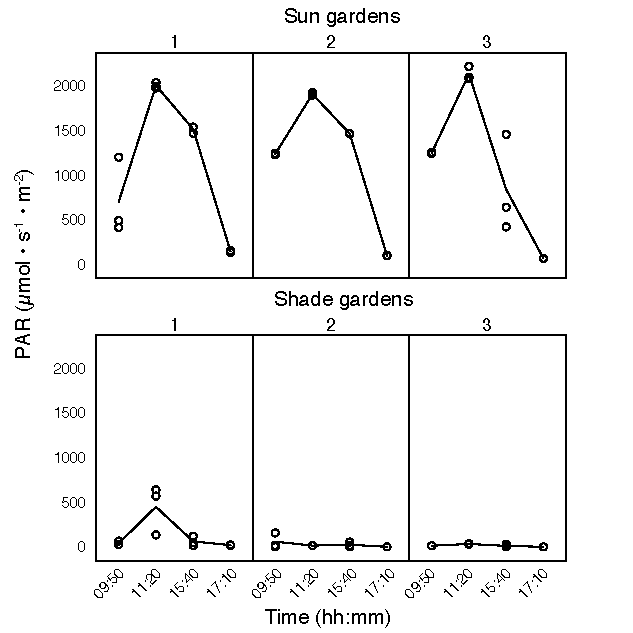
\includegraphics[scale=0.75]{par}
\caption{Photosynthetically active radiation (PAR) measurements for the six common garden sites showing daily natural variation in light abundance. Line depicts mean of three measurements per time point per garden.}
\label{par}
\end{figure}

\clearpage

%%% TABLE S1: SITE CHARACTERISTICS
\begin{table}[htdp]
\tiny
\caption{Habitat characteristics of rhizome collection sites.}
\centering
\begin{tabu} to \textwidth {X[0.33]XX[2.25]X[2.35]X[0.75]XXXXX}
\toprule
Site & Date collected$^{1}$ & Lat. & Long. & Elev. (m) & Soil type & Habitat & PAR$^2$ & \% open & $\bar{dbh}$ (cm) \\
\midrule
1 & 10 Jul & 39.0050602776535 & -106.943317166893 & 3461 & Very Wet & Sun & 1980 & 99.84 & 0 \\
2 & 10 Jul & 38.9885304491745 & -106.945774321867 & 3218 & Moist Loamy & Shade & 300 & 6.76 & 10 \\
3 & 11 Jul & 38.9900162385746 & -106.944210201638 & 3240 & Moist Loamy & Shade & 130 & 8.06 & 121.75 \\
4 & 11 Jul & 38.9900829890862 & -106.943450029132 & 3253 & Very Wet & Sun & 2030 & 82.94 & 0 \\
5 & 11 Jul & 38.9896982273227 & -106.9432894133 & 3261 & Very Wet & Sun & 2034 & 95.42 & 0 \\
6 & 11 Jul & 38.9897805369006 & -106.94429611421 & 3244 & Moist Loamy & Shade & 130 & 4.16 & 83.25 \\
7 & 11 Jul & 38.9890385630266 & -106.944483622637 & 3220 & Very Wet & Sun & 2134 & 99.84 & 0 \\
8 & 11 Jul & 38.9876108211294 & -106.944190554921 & 3250 & Moist Loamy & Shade & 28 & 3.38 & 81.75 \\
9 & 12 Jul & 38.9607056556777 & -106.973679741745 & 3023 & Very Wet & Sun & 2026 & 88.14 & 0 \\
10 & 12 Jul & 38.9600423351315 & -106.973476684125 & 3013 & Wet Loamy & Shade & 35 & 5.72 & 72.25 \\
11 & 12 Jul & 38.9609507737634 & -106.973571138078 & 3994 & Very Wet & Sun & 1933 & 86.84 & 0 \\
12 & 12 Jul & 38.9655594715881 & -106.968516958823 & 3994 & Very Wet & Shade & 32 & 3.9 & 101 \\
13 & 13 Jul & 38.9828665210329 & -106.989822099201 & 4058 & Very Wet & Sun & 1780 & 96.2 & 0 \\
14 & 13 Jul & 38.9774145794955 & -106.98986568487 & 4082 & Very Wet & Sun & 1870 & 88.4 & 0 \\
15 & 13 Jul & 38.9771831850899 & -106.989697600334 & 4057 & Very Wet & Sun & 1850 & 99.84 & 0 \\
16 & 13 Jul & 38.976356744414 & -106.990078474138 & 4052 & Very Wet & Shade & 54 & 4.68 & 98 \\
17 & 13 Jul & 38.975757817399 & -106.990327194402 & 4046 & Moist Loamy & Shade & 60 & 4.16 & 140.5 \\
18 & 13 Jul & 38.974195183581 & -106.989498527449 & 4051 & Very Wet & Shade & 40 & 7.28 & 78.75 \\
\bottomrule
\multicolumn{4}{l}{$^{1}$All collections made in 2011.} & & & & & \\
\multicolumn{4}{l}{$^{2}$PAR units = $\mu \text{mol} \times s^{-1} \times m^{-2}$} & & & & & \\
\end{tabu}
\label{tableS1}
\end{table}

\newpage


%%% TABLE S2: 
\begin{table}[htdp]
\small
\caption{Environmental attributes of sun and shade source sites used in field common gardens.}
\centering
\begin{tabu} to \textwidth {X[1.5]XXXXXX}
\toprule
& \multicolumn{2}{l}{sun sites ($n = 9$)} & \multicolumn{2}{l}{shade sites ($n = 9$)} & \multicolumn{2}{l}{ANOVA} \\
\cline{2-7}
attribute & $\mu$ & $se$ & $\mu$ & $se$ & $F$ & $p$ \\
\midrule
PAR$^1$ & 1959.7 & 37.0 & 89.0 & 29.4 & 1564 & $<10^{-4}$ \\
\% open & 93.1 & 2.2 & 5.3 & 0.6 & 1527 & $<10^{-4}$ \\
dbh (cm) & 0.00 & 0.00 & 87.5 & 12.2 & 51.77 & $<10^{-4}$ \\
elevation (m) & 3601 & 146 & 3568 & 150 & 0.025 & 0.875 \\
\bottomrule
\multicolumn{4}{l}{$^{1}$PAR units = $\mu \text{mol} \times s^{-1} \times m^{-2}$} & & &\\
\end{tabu}
\label{tableS2}
\end{table}



\vspace{2cm}


\begin{table}[htdp]
\small
\caption{Environmental attributes of sun and shade source sites used in greenhouse experiment ($n=37$ plants total.)}
\centering
\begin{tabu} {X[0.3]X[1.3]X[1.5]X[0.8]X[0.7]X[0.7]X[0.75]X[0.6]}
\toprule
site$^{1}$ & lat. & long. & elev. (m) & source & \% open & $n$ shade$^2$ & $n$ sun$^2$ \\
\midrule
8 & 38.977172541 & -106.992202530 & 3049 & shade & 13.52 & 3 & 4\\
11 & 38.977208673 & -106.991636863 & 3049 & shade & 9.36 & 2 & 2\\
19 & 38.960075121 & -106.973484675 & 3007 & shade & 32.24 & 4 & 3\\
12 & 38.974598748 & -106.990864137 & 3044 & sun & 96.72 & 4 & 5\\
13 & 38.974504757 & -106.990819289 & 3045 & sun & 84.24 & 6 & 4\\
\bottomrule
\multicolumn{8}{l}{$^{1}$Site numbers do not correspond to those listed in Table S1.}\\
\multicolumn{8}{l}{$^{2}$Numbers correspond to $n$ plants grown from seed under the given light treatment.}\\
\end{tabu}
\label{tableS3}
\end{table}


\clearpage

\section{Regression modeling approach}

\subsection{Regression model form}
We consider a hierarchical regression model that estimates effects of clone, genet, source type, as well as the environmental effects of garden plot and garden type, on focal plant phenotypes:

%%%% eq1
\begin{equation} \label{eq1}
y^{k}_{j(i)} = \alpha^{k}_{j(i)} + \beta^{k}_{l}\\
\end{equation}

The response variable $y^{k}_{j(i)}$ is the plant trait we wish to model, for clone $i$ nested within genet $j$ from source type $k$. The first term on the right-hand side of Eq. 1 collects all of the constitutive effects, while the second term models the environmental effects of growth in different common gardens. (Note that superscripts $k$ denote group-level indexes and are \emph{not} exponents). We can expand the constitutive effects terms as follows:

%%%% eq2
\begin{equation} \label{eq2}
\alpha^{k}_{j(i)} = \alpha_{j} + \alpha_{1}S_{s} + \varepsilon_{i}
\end{equation}
\begin{align*}
\alpha_{j} &\sim \mathcal{N}(\alpha_{0}, \tau^2_{\alpha(j)}) \\
\varepsilon_{i} &\sim \mathcal{N}(0, \sigma^{2}_{e})
\end{align*}

Eq. 2 captures observation-level residual variance ($\varepsilon_{i}$), among-genet differences ($\alpha_{j}$), and a population-level (i.e. fixed) effect of source type ($\alpha_{1}S_{s}$), where $S_{s}$ is an indicator variable that equals 1 if source type is 'sun' and equals 0 otherwise. Thus, $\alpha_0$ is the population-level intercept for plants derived from shade source habitats measured in shaded gardens (the 'reference' level).

The second term on the right hand side of Eq. 1 captures the effects of environmental variation induced by growth across the six common gardens, as well as the average effect of growing in the sun-type gardens:

%%%% eq3
\begin{equation} \label{eq3}
\beta^{k}_{l} = \beta_{l} + \beta_{1}S_{s}S_{g}
\end{equation}
\begin{align*}
\beta_{l} &\sim \mathcal{N}(\beta_{j}S_{g},\tau^2_{\beta(l)}) \\
\beta_{j} &\sim \mathcal{N}(\beta_{0}, \tau^{2}_{\beta(j)})
\end{align*}

Eq. 3 captures plot-to-plot differences among gardens, $\beta_{l}$, which is itself influenced by the main effect of growing in the sun gardens, $\beta_0$, as well as genet-specific effects of growing in sun gardens, $\beta_{j}$. When estimated, this latter term represents a random slope term where the overall slope $\beta_0$ is perturbed with a variance given by $\tau^{2}_{\beta(l)}$. $S_g$ is an indicator variable that equals 1 if the common garden plot is in the sun and 0 if it is in the shade. Thus, $\beta_l$ is constructed so that the expected value ($\beta_{j}S_{g}$) equals 0 in shade gardens, contributing only plot-to-plot level effects given by the variance term $\tau^2_{\beta(l)}$. $\beta_0$ estimates the population-level (main) effect of growth in sun gardens, while $\beta_{1}S_{s}S_{g}$ captures the extent to which sun source plants differ in their response from the main effect $\beta_0$ of growing in the sun, with $S_s$ again indicating source type, as in Eq. 2 above. For all focal plant traits, we initially consider a reduced model where we remove the random slope effect for genet, simplifying the structure of $\beta_{l}$ and estimating one fewer parameter ($\tau^2_{\beta(j)}$):
$$\beta_{l} \sim \mathcal{N}(\beta_0S_{g},\tau^2_{\beta(l)})$$

Models were fit via restricted maximum likelihood with and without this term and compared with a likelihood ratio test.

To summarize, the population-level terms to be estimated are:
\begin{itemize}
\item $\alpha_0$: Intercept-level term for shade source plants in shade gardens.
\item $\alpha_1$: Effect of source type = sun on constitutive phenotype.
\item $\beta_0$: Average main effect of sun garden on phenotype for shade-derived plants.
\item $\beta_1$: Differential effect of sun gardens when source type = sun (source type $\times$ garden type interaction).
\end{itemize}

The group-level terms to be estimated are:
\begin{itemize}
\item $\tau^2_{\alpha(j)}$: genet-level variance in constitutive intercept; single term for both source types ($n = 18$ genets).
\item $\tau^2_{\beta(l)}$: garden plot-level variance in phenotype ($n=6$ garden plots in total)
\item $\tau^2_{\beta(j)}$: In the fully parameterized model, this term estimates the magnitude of the among-genet variance in the response to growing in sun gardens. In the reduced form, this term is not estimated.
\item $\sigma^2_{e}$: i.i.d observation- (i.e. clone-) level residual variance.
\end{itemize}

\subsubsection{Addition of covariates}

We including trait covariates into our models to control for underlying differences in correlated characters as well as to test whether a main effect of source habitat manifests as different quantitative relationships between traits (e.g. leaf mass vs. leaf area), rather than simply a difference in the average location of residuals once a covariate is taken into account. Thus, we estimate additional $\gamma_{w}$ parameters for each level of the relevant source habitats and/or garden types. In these cases, our model for the effect of a covariate $x_i$ on phenotype $y$ becomes (dropping the $w$ subscript for simplicity):


%%%% eq. 4
\begin{equation} \label{eq4}
y^{k}_{j(i)} = \gamma^{k}_{g} x_{i} + \alpha^{k}_{j(i)} + \beta^{k}_{l}
\end{equation}
\begin{align*}
\gamma^{k}_{g} = \gamma_{0} + \gamma_{1}S_{g} + \gamma_{2}S_{s} + \gamma_{12}S_{g}S_{s}
\end{align*}

where $\gamma_{0}$ is the overall slope for shade-source plants measured in shade gardens, $\gamma_{1}$ is the difference in the slope when the $S_{g}$ garden-type indicator variable equals 1, $\gamma_{2}$ is the difference in the slope when the $S_s$ source-type indicator variable equals 1, and $\gamma_{12}$ is the difference when the product $S_{g}S_{s}$ equals 1 (i.e. a three-way interaction term). When only $\gamma_0$ appears in the model, this term is the average value of the covariate across all plants and not just for the reference level.

\newpage

%%%% SECTION 3 %%%%
\section{Supplemental analysis of plant morphological traits}
\subsection{Untransformed traits}
\subsubsection{Trait distributions}
Below we present the distributions of, and correlations between, raw trait data for plant size as indicated by number of leaves ('leaf number'), leaf dry mass (g), leaf area (cm$^2$), and petiole length (mm), as well as the results from an analysis of each trait without accounting for underlying differences in plant size or leaf mass. Such an analysis is meant to quantify 'face-value' differences and not to compare investment in petiole elongation nor leaf expansion, which we deal with in detail in the main text.

\vspace{2cm}

%%%% Fig. S4 %%%%
% raw trait values
\begin{figure}[h]
\centering
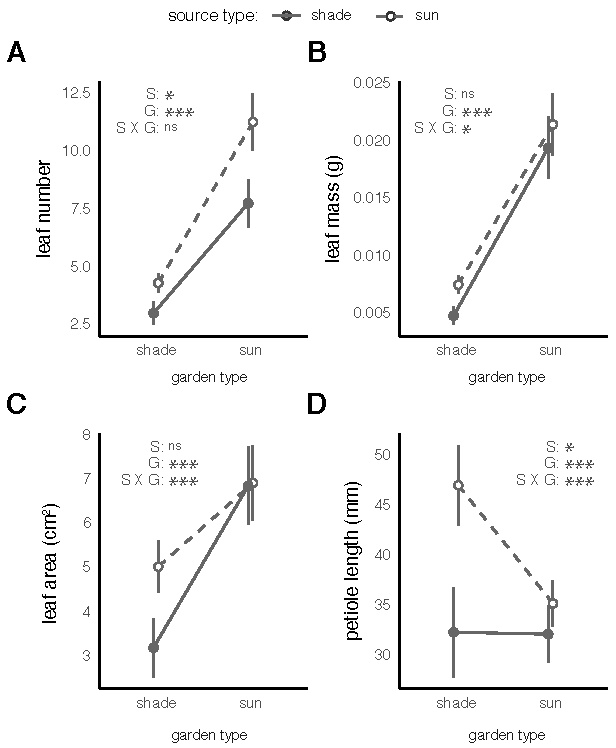
\includegraphics[scale=0.8]{ESM_raw_data_v2}
\caption{Average raw trait values ($\pm$ 95\% confidence intervals) across garden types broken down by source habitat type. Regression analyses (see Tables S4 and S5 for results) used $\text{log}_{10}$-transformed values for (\textbf{A}) leaf number, (\textbf{B}) leaf dry mass, (\textbf{C}) and leaf area ($\text{cm}^{2}$), while (\textbf{D}) petiole length (mm) was analyzed on the linear scale. 'S' = source effect, 'G' = garden type effect, and 'S $\times$ G' = source-by-garden effect (Table S5).}
\label{FigS4}
\end{figure}

\clearpage

%%%% Fig. S5 %%%%
% trait pairwise correlations plot
\begin{figure}[!hptb]
\centering
\includegraphics[scale=0.66]{traitcors}
\caption{Correlation among measured plant traits, colored by garden type (gray = shade, blue = sun). 'Cor' indicates Pearson's $r$ correlation coefficient for all data, while 'sun' and 'shade' indicate $r$ calculated separately for sun and shade gardens, for each pair of traits. Diagonal plot elements depict single trait distributions, again broken down by garden type. Leaf number, leaf area, and leaf mass are $\text{log}_{10}$-transformed.}
\label{FigS5}
\end{figure}

\clearpage

\subsubsection{Model results}

Below are model coefficient estimates produced for un-transformed traits as well as results of a model of leaf mass (log g dry mass) that includes log leaf number as a covariate (Table S4) and ANOVA-style hypothesis tests for marginal effects of fixed model terms (Table S5).

\vspace{1cm}

% TABLE S4
\begin{table}[!htp]
\small
\caption{Supplementary coefficient estimates for models of plant traits.}
\centering
\begin{tabular}{lllll}
\toprule
coefficient & sym$^1$ & (log) leaf num & (log g) dry leaf mass & (log g) dry leaf mass$^2$ \\
\midrule
intercept [shade] & $\alpha_0$ & $0.4 (0.27, 0.53)^{***}$ & $-2.4 (-2.52, -2.28)^{***}$ & $-2.6 (-2.7, -2.51)^{***}$ \\
source [sun] & $\alpha_1$ & $0.17 (0.05, 0.28)^{**}$ & $0.19 (0.07, 0.32)^{***}$ & $0.11 (0.01, 0.21)\cdot$ \\
garden [sun] & $\beta_0$ & $0.39 (0.23, 0.55)^{**}$ & $0.6 (0.46, 0.73)^{***}$ & $0.39 (0.28, 0.5)^{***}$ \\
source [sun]$\times$garden [sun] & $\beta_1$ & $0 (-0.1, 0.1)$ & $-0.16 (-0.27, -0.04)^{**}$ & $-0.16 (-0.26, -0.05)^{***}$ \\
covariate (leaf num.) & $\gamma_0$ &  &  & $0.51 (0.4, 0.63)^{***}$ \\
genet & $\tau_{\alpha(j)}$ & $0.09 (0.05, 0.14)$ & $0.09 (0.04, 0.14)$ & $0.06 (0.02, 0.1)$ \\
garden plot & $\tau_{\beta(l)}$ & $0.09 (0.04, 0.16)$ & $0.07 (0.02, 0.12)$ & $0.04 (0, 0.08)$ \\
residual error & $\sigma_{e}$ & $0.2 (0.18, 0.22)$ & $0.23 (0.21, 0.25)$ & $0.21 (0.19, 0.22)$ \\
$R^{2}_{m}$ &  & 0.43 & 0.5 & 0.62 \\
$R^{2}_{c}$ &  & 0.6 & 0.59 & 0.66 \\
 &  &  &  &  \\
 \midrule
 coefficient & sym$^1$ & (log cm$^2$) leaf area & petiole length (mm) & \\
 \midrule
intercept [shade] & $\alpha_0$ & $0.42 (0.3, 0.54)^{***}$ & $33.44 (24.41, 42.56)^{***}$ & \\
source [sun] & $\alpha_1$ & $0.2 (0.08, 0.31)^{***}$ & $13.12 (8.05, 18.24)^{***}$ & \\
garden [sun] & $\beta_0$ & $0.33 (0.18, 0.48)^{**}$ & $-2.54 (-15.19, 10.04)$ & \\ 
source [sun]$\times$garden [sun] & $\beta_1$ & $-0.2 (-0.31, -0.09)^{***}$ & $-9.48 (-15.86, -3.28)^{***}$ & \\ 
genet & $\tau_{\alpha(j)}$ & $0.08 (0.04, 0.13)$ & $1.64 (0, 4.21)$ & \\
garden plot & $\tau_{\beta(l)}$ & $0.08 (0.03, 0.14)$ & $7.59 (3.46, 12.72)$ & \\
residual error & $\sigma_{e}$ & $0.22 (0.2, 0.24)$ & $12.57 (11.53, 13.73)$ & \\
$R^{2}_{m}$ &  & 0.19 & 0.15 & \\
$R^{2}_{c}$ &  & 0.36 & 0.38 & \\
\bottomrule
\multicolumn{5}{l}{$\cdot0.05<p<0.1$, $*p<0.05$, $**p<0.01$, $***p<0.001$ (see Methods)}\\
\multicolumn{5}{l}{95\% confidence intervals calculated via likelihood profiling.} \\
\multicolumn{5}{l}{$^{1}$See section 2.1 for symbolic representation of model coefficients in context of regression model.} \\ 
\multicolumn{5}{l}{$^{2}$Model included log leaf number as covariate.} \\
%\end{tabu}
\end{tabular}
\label{tableS4}
\end{table}

\newpage


% TABLE S5
\begin{table}[htp]
\small
\caption{Supplementary ANOVA-style hypothesis tests for individual model terms.}
\centering
\begin{tabular}{lllll}
\toprule
Response & Model term & MSE$^1$ & $F$ & \emph{P-value}\\
\midrule
($\text{log}$) leaf num & source & 0.43 & $F(1,15.2) = 10.9$ & 0.005\\
 & garden & 0.94 & $F(1,4.1) = 23.8$ & 0.008\\
 & source $\times$ garden & 0 & $F(1,256.0) = 0$ & 0.98\\
  & & & &\\
($\text{log g}$) dry leaf mass & source & 0.23 & $F(1,15.2) = 4.5$ & 0.05\\
 & garden & 3.56 & $F(1,4.1)$ = 69.1 & 0.001\\
 & source $\times$ garden & 0.38 & $F(1,257.2) = 7.4$ & 0.007\\
& & & &\\
($\text{log g}$) dry leaf mass & source & 0.02 & $F(1,17.6) = 0.4$ & 0.532\\
 & garden & 1.67 & $F(1,8.0) = 39.7$ & $<0.001$\\
 & source $\times$ garden & 0.38 & $F(1,259.0) = 9$ & 0.003\\
 & log leaf number & 3.05 & $F(1,247.1)$ = 72.5 & $<0.001$\\
& & & &\\
($\text{log cm}^{2}$) leaf area & source & 0.17 & $F(1,15.2) = 3.7$ & 0.074\\
 & garden & 0.5 & $F(1,4.1) = 10.7$ & 0.03\\
 & source $\times$ garden & 0.61 & $F(1,257.0) = 13$ & $<0.001$\\
& & & &\\
petiole length (mm) & source & 3342 & $F(1,15.3) = 21.1$ & $<0.001$\\
 & garden & 204 & $F(1,4.0) = 1.3$ & 0.319\\
 & source $\times$ garden & 1376 & $F(1,260.8) = 8.7$ & 0.003\\
\bottomrule
\multicolumn{5}{l}{$^{1}$Mean squared error.} \\ 
\end{tabular}
\label{tableS5}
\end{table}

\vspace{1cm}

\subsection{Traits modeled with covariates}
The content in this section relates to analyses of focal plant traits where relevant covariates were considered, in addition to cases where response variables and covariates had been transformed via orthogonalization by linear regression with our metric of plant size (log leaf number) and leaf mass (log g dry mass) (see Methods). 

%%% FIG S6 %%%
% hypothesized covariate interactions with leaf traits
\begin{figure}[!h]
\centering
\includegraphics[scale=0.7]{FigS7covrawplots}
\caption{Hypothesized covariate interaction plots suggest source type and garden type impact relationships among plant traits. Depiction of such patterns in this manner reflects our regression modeling approach (see Methods). Plotted are trait values for all $n=274$ plants where linear regression slopes ($\pm$ 95\% confidence intervals) have been plotted over the raw data to indicate trends in the data. Model results for (\textbf{A}) leaf number and leaf mass as response variables are listed in \S 3.4 below. \textbf{B}. '(res)' indicates residual vector of log leaf mass ($x$-axis) or log leaf area ($y$-axis) orthogonalized against log leaf number. \textbf{C}. '(res)' indicates the same orthogonalization as in \textbf{C} above, but for petiole length along the $y$-axis. \textbf{D}. '(res)' indicates residual vector of log leaf area ($x$-axis) or petiole length ($y$-axis) orthogonalized against log leaf number and log leaf mass.}
\label{FigS6}
\end{figure}

\clearpage

%%% FIG S7 %%%
% marginal effects plots for leaf area and petiole length
\begin{figure}[h]
\centering
\includegraphics[scale=0.6]{Morphology_effects_breakdown_panel_3}
\caption{Plots of marginal effects of source and garden type from regression models (see Table 1, main text for results). \textbf{A}. Main source $\times$ garden type effects depicted for leaf area, with post-hoc source and garden-type contrasts shown in \textbf{B}, indicating where significant differences occurred. Levels ($x$-axis categories) indicate the particular contrasts plotted per column, with the difference between distinct source and garden type combinations plotted on the $y$-axis. \textbf{C}. Marginal effect of the leaf mass covariate interaction with source and garden type is depicted, such that the difference between source types depends both on garden type as well as the mass of the leaf considered. \textbf{D}. Post-hoc inspection of source $\times$ garden effect (averaged over the covariate) show significant focal contrasts between source types in shade gardens (see Tables 1 and 3, main text, for model results [petiole length 'A']). \textbf{E}. Marginal effects of the leaf area covariate interaction with source and garden type is depicted, showing increased residual petiole elongation as a function of leaf expansion for sun-derived plants grown in shade. \textbf{F}. In contrast to plots in panels \textbf{C--D}, no source $\times$ garden type main effects remained over and above the leaf expansion covariate (see Tables 1 and 3, main text, for model results [petiole length 'B']).}
\label{FigS7}
\end{figure}

\clearpage

\subsection{Analysis of plant size and leaf mass}

\subsubsection{Leaf number} Using log transformed values (unless otherwise noted), we tested for effects of source habitat and garden habitat on plant vegetative traits. Of these, sun-source plants had 40\% more leaves than shade-source plants in both sun and shade gardens (Fig. 1A, $\alpha_{1}= 0.17 [0.05, 0.28]$, $p < 0.05$, Table 1; overall source effect $p=0.005$, Table 3), and plants from both source habitats had nearly twice as many leaves in sun gardens as they did in shade gardens ($\beta_{0} = 0.39 [0.23, 0.55]$, $p<0.001$, Table 1; overall garden effect $p=0.008$, Table 3). We tested for but detected no interaction between source and garden type, and this term was dropped from the reported model with no change in coefficient estimates or in the estimated $R^{2}_{m}$ of the marginal model, which remained at ~40\% (Table 1). Post-hoc comparisons of all source and garden contrasts can be found in Fig. S8.

\subsubsection{Leaf mass} Using log transformed values (unless otherwise noted), we next assessed whether investment in dry mass of the largest leaf, as a function of plant size (leaf number) and garden type, varied between source types (see Fig. S6A for plots of hypothesized covariate interactions). We found that leaf number positively predicted leaf mass similarly across source and garden types ($\gamma_{0} = 0.51 [0.4, 0.6]$, $p<0.001$, Table 1). Importantly, the way plants invested in leaf mass in sun and shade gardens differed by source type (source $\times$ garden overall effect $p=0.003$, Table 3). Specifically, when grown in shade gardens, sun-source plants had a marginally significant 28\% increase in leaf mass over shade-source plants (Fig 1B), independent of leaf number ($\alpha_{1} = 0.11 [0.01, 0.21]$, $0.05\leq p<0.1$, Table 1; see Fig. S8B for plot of marginal effects). In sun gardens, plants of both sources did not differ (post-hoc comparison $p>0.05$, Fig. S8). Accordingly, the higher leaf mass in sun gardens was less extreme for sun-source compared to shade-source plants, decreasing from from 2.5-fold to 1.7-fold (~30\%) ($\beta_{1}= -0.16 [-0.26, -0.05]$, $p<0.001$, Table 1). Fixed effects explained $>60\%$ of the variation in the data for the model of leaf mass reported in Table 1.

%%% FIG S8 %%%
% marginal effects plots for leaf number and leaf mass
\begin{figure}[!htbp]
\centering
\includegraphics[scale=0.8]{Morphology_effects_breakdown_panel}
\caption{Marginal effects plots for leaf number and leaf mass. \textbf{A--B}. Source types exhibit consistent differences in log leaf number (our metric of plant size) across both garden types. \textbf{C--D}. Leaf mass, after accounting for the effects of plant size, showed a significant source $\times$ garden type effect, which manifested in post-hoc contrasts (\textbf{D}) as elevated leaf mass for sun-source compared to shade-source plants in shade gardens. Model results are given in Tables S4 and S5.}
\label{FigS8}
\end{figure}

\clearpage

%%%% SECTION 4 %%%%
\section{Supplementary analysis of plant defenses and herbivore resistance}
\subsection{Glucosinolates}
\subsubsection{Weighted pooling approach}
Glucosinolate (GSL) concentrations were pooled into three distinct chemical classes, designated as IYG and OYG, which refer to GSL compounds yielding isothiocyanates (IYG) or oxazolidine-2-thiones (OYG) upon tissue disruption, as determined in bittercress by Louda and Rodman (1983a) and Rodman and Louda (1985). $m/z$ is the mass-to-charge ratio of the GSL precursor ions quantified in this study. Retention time (RT) indicates the time in minutes when peak intensity of a given compound was observed. GSL concentrations were quantified as parent ion counts per gram of wet leaf material and multiplied by the weighting factors given below (Table S6) to obtain approximate relative abundances (i.e., mg of focal IYG compound per mg total IYG; see Methods).

Three peaks with  $m/z = 390$, the parent ion corresponding to 1-(hydroxymethyl)propyl GSL, were observed (Table S6). 1-(hydroxymethyl)propyl GSL could not be definitively assigned to a single peak using our methods. Because intensities of the three peaks were correlated across samples, the peak at RT = 7.3 mins (which achieved high chromatographic resolution) was used for quantification of 1-(hydroxymethyl)propyl GLS parent ion counts. 2-(hydroxymethyl)propyl GSL, another compound with $m/z = 390$, was previously identified in bittercress (Louda and Rodman 1983a). However, because the non-hydroxylated form of this GSL is present at relatively low amounts, we did not quantify this compound in this study.

\vspace{1cm}

%%%% TABLE S6 %%%%
\begin{table}[!h]
\small
\caption{Glucosinolate detection and pooling weights.}
\centering
\begin{tabular}{llllll}
\toprule
Name & Short name & Class & $m/z$ & RT (minutes) & Weighting factor\\
\midrule
2-phenethyl & Phe & IYG & 422 & 12.5 & 1.987\\
benzyl & Ben & IYG & 408 & 10.6 & 4.062\\
1-methylethyl & iPro (isopropyl) & IYG & 360 & 7 & 0.205\\
2-methylpropyl & iBut (isobutyl) & IYG & 374 & 8.9 & 2.74\\
1-methylpropyl & sBut (sec-butyl) & IYG & 374 & 9.2 & 0.777\\
2-hydroxy-2-phenethyl & hPhe & OYG & 438 & 10.1 & NA\\
1-(hydroxymethyl)ethyl & hiPro & OYG & 376 & 4.2 & NA\\
1-(hydroxymethyl)propyl & hsBut & OYG & 390 & 4.6, 6.3, 7.3 & NA\\
indole-3-ylmethyl & I3M & indole & 447 & 11.5 & NA\\
\bottomrule
\end{tabular}
\label{tableS6}
\end{table}

\newpage

%%% FIG S9 %%%
% post-hoc marginal effects for total amounts of IYG, I3M
\begin{figure}[!hptb]
\centering
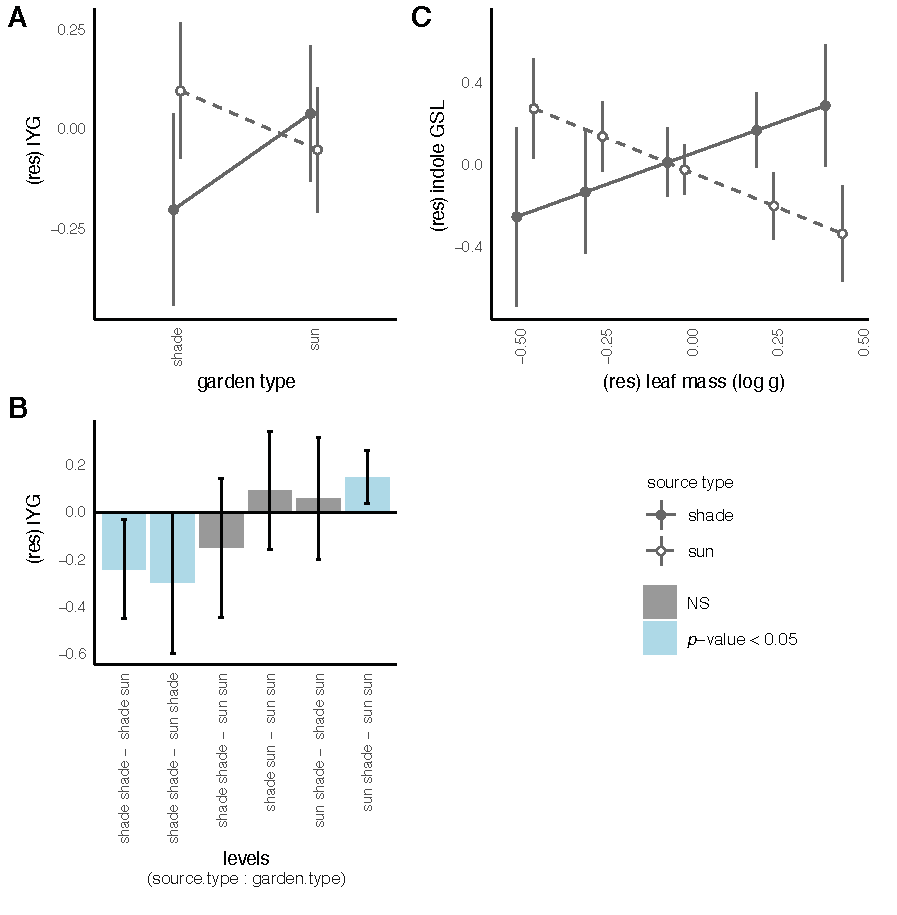
\includegraphics[scale=0.8]{GLS_effects_breakdown_panel}
\caption{Marginal effects plots for isothiocyanate-yielding glucosinolates (IYG; \textbf{A--B}) and indole glucosinolate (I3M; \textbf{C}) across common garden plants. \textbf{A}. source $\times$ garden type interaction is depicted of IYG concentrations after orthogonalization against plant size (i.e. log leaf number; see Methods). \textbf{B}. Post-hoc contrasts indicate elevated IYG for sun-source plants relative to shade-source plants in shade gardens. This was driven by opposite effects of shading on IYG for each source type: sun-source plants accumulated more IYG, and shade-source plants accumulated less, in shade gardens compared to sun gardens. \textbf{C}. Marginal effects plot showing covariate interaction between (log) g wet leaf mass and indole concentration, revealing that sun and shade source plants exhibited contrasting patterns of indole concentration as a function of leaf mass. In this analysis, both the covariate and response variable have been orthogonalized against plant size (see Methods).}
\label{FigS9}
\end{figure}


%\newpage
\clearpage
\subsubsection{Principal components analysis}
Data were $\text{log}_{10}$-transformed, mean-centered and scaled GSL concentrations for eight individual compounds (see Table S 6 and Methods for details). The first three principal components explained 67\% of the variation in the data. Source site information corresponds to that depicted in Fig. S2 and listed in Table S1 (\S1).

\vspace{2cm}

%%% FIG S10 %%%
% PCA with PC1 vs. PC2, and PC3 vs. PC2
\begin{figure}[!hptb]
\centering
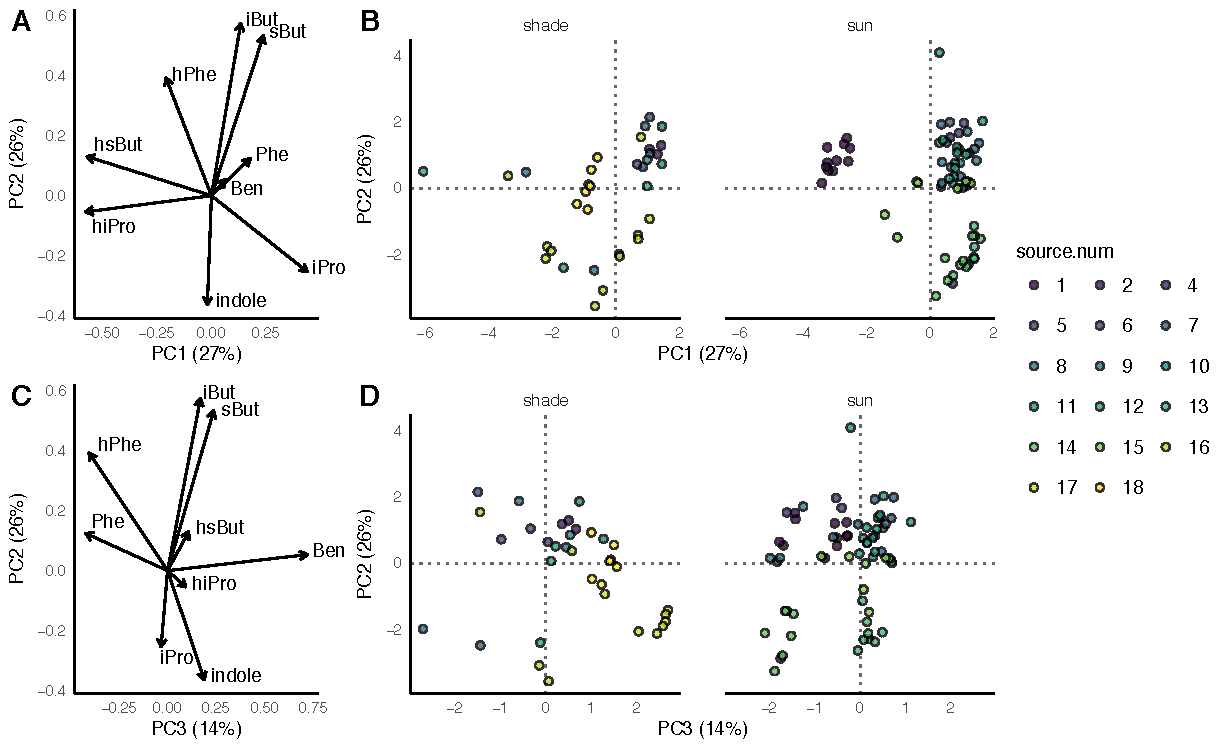
\includegraphics[scale=0.75]{gls_PCA}
\caption{Principal components analysis of eight individual GSL reveals differentiation based on source location (i.e. genet) seen in plots of  PC1 vs PC2 (\textbf{A--B}) and PC2 vs PC3 (\textbf{C--D}), broken down by source type. }
\label{FigS10}
\end{figure}


\clearpage


\subsection{Operational herbivore resistance}
Data are mass of $n=156$ larvae after feeding for 48 h on common garden plants (see Methods).

\vspace{2cm}

%%% FIG S11 %%%
%PCA with PC1 vs. PC2, and PC3 vs. PC2
\begin{figure}[!htbp]
\centering
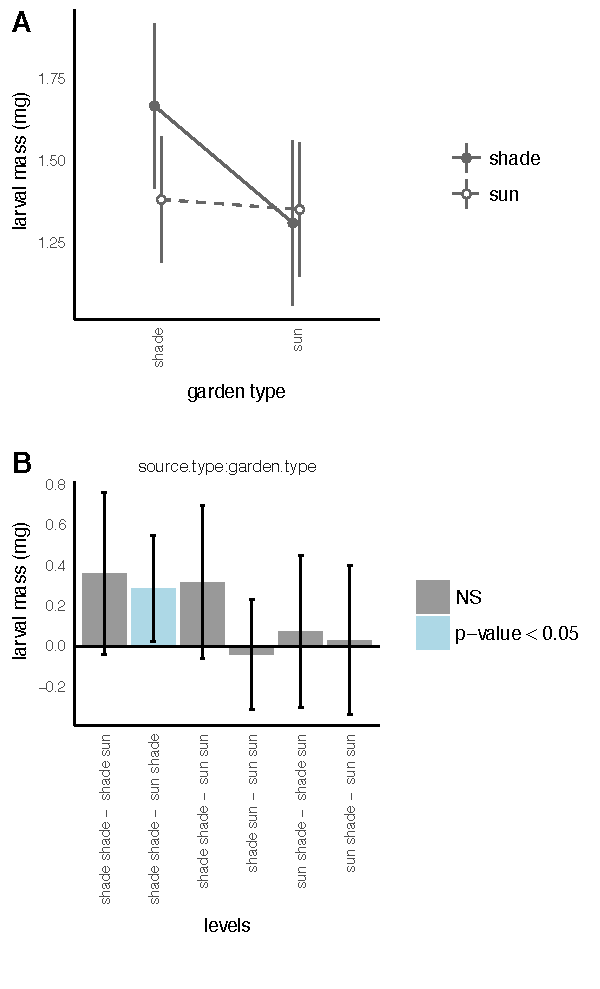
\includegraphics[scale=0.8]{larm_effects_breakdown}
\caption{Marginal effects plots depicting source $\times$ garden interaction (\textbf{A}), where post-hoc contrasts indicate elevated larval mass on shade-derived plants relative to sun-derived plants in shade gardens (\textbf{B}).}
\label{FigS11}
\end{figure}


\clearpage

%%%% SECTION 5 %%%%
\section{Analysis of greenhouse experiment}
\subsection{Model form}
We estimated coefficients in a hierarchical regression model of the following form:

%%%% eq5
\begin{equation} \label{eq5}
y^{g}_{kji} = \alpha^{g}_{kj} + \beta S_{l} + \gamma x_{i} + \varepsilon_{i}
\end{equation}
\begin{align*}
\alpha^{g}_{kj} &\sim \mathcal{N}(\alpha_{kj}, \tau^{2}_{g})\\
\alpha_{kj} &\sim \mathcal{N}(\alpha_0 + \alpha_{j}, \tau^2_{k}) \\
\alpha_{j} &\sim \mathcal{N}(0, \tau^2_{j}) \\
\varepsilon_{i} &\sim \mathcal{N}(0, \sigma^{2}_{e})
\end{align*}

Where $y^{g}_{kji}$ is the trait measure (either log cm$^2$ leaf area or mm petiole length) of leaf $i$ from position $j$ from plant $k$ from genetic family $g$. $\alpha_0$ is the intercept of the reference level (shade environment), $\beta$ is the slope of the average response to growth in elevated FR:R light ('sun'), where $S_{l}$ is an indicator variable for light environment that equals $0$ in simulated shade and $1$ in the sun environment. Finally, $\gamma$ is the slope of the increase in petiole length per unit increase in the value of covariate $x$. We model variation among families, among plants (nested within family), and among leaf positions as a series of group-level (i.e. random) effects, similar to Eqs. 1 and 4 above. Our model of leaf area did not include estimation of a $\gamma$ covariate term.

\subsection{Model results and marginal effects plots.}
Below are are results for $n=37$ plants reared from seed in the greenhouse.

\vspace{1cm}

%%% TABLE S7
\begin{table}[!h]
\small
\caption{Coefficient estimates for greenhouse experiment.}
\centering
\begin{tabular}{llll}
\toprule
Estimate & sym. & log leaf area (cm$^2$) & petiole length (mm)\\
\midrule
Intercept [shade] & $\alpha_0$ & 0.82 (0.57, 1.08)$^{***}$ & 21.56 (14.15, 28.9)$^{***}$\\
light condition [sun] & $\beta$ & 0.38 (0.29, 0.46)$^{***}$ & -25.9 (-31.04, -20.82)$^{***}$\\
covariate$^1$ & $\gamma$ & NA & 52.82 (46.42, 59.94)$^{***}$\\
family ID & $\tau_g$ & 0.11 (0.05, 0.27) & 4.05 (0, 9.09)\\
plant ID & $\tau_k$ & 0.1 (0.07, 0.14) & 5.92 (4.02, 8.14)\\
leaf position & $\tau_j$ & 0.21 (0.1, 0.45) & 1.18 (0, 3.88)\\
residual error & $\sigma_{e}$ & 0.13 (0.11, 0.15) & 6.93 (6.05, 8.01)\\
$R^2_m$ & & 0.3 & 0.67\\
$R^2_c$ & & 0.86 & 0.84\\
\bottomrule
\multicolumn{4}{l}{$^1$ Covariate for petiole length model was log leaf area (cm$^2$)}
\end{tabular}
\label{tableS7}
\end{table}

\vspace{2cm}

%%% TABLE S8
%%% ANOVA style results for greenhouse experiment %%%
\begin{table}[!h]
\small
\caption{ANOVA-style hypothesis tests for individual model terms in greenhouse analysis.}
\centering
\begin{tabular}{lllll}
\toprule
Response & Model term & MSE & $F$ & $P$-value\\
\midrule
log leaf area (cm$^2$) & light condition & 1.4 & $F(1,31)$ = 82.3 & $<0.001$\\
 &  &  &  & \\
petiole length (mm) & log leaf area (cm$^2$) & 8320 & $F(1,10) = 173.1$ & $<0.001$\\
 & light condition & 4243 & $F(1,38) = 88$ & $<0.001$\\
\bottomrule
\end{tabular}
\label{tableS8}
\end{table}

\vspace{2cm}

%%% FIG S12 %%%
% marginal effects plot for greenhouse phenotypes
\begin{figure}[!hptb]
\centering
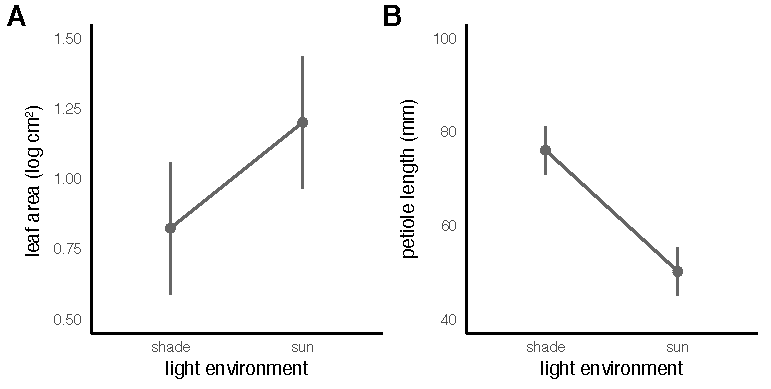
\includegraphics[scale=0.8]{GHareapetlen}
\caption{Marginal effects means ($\pm 95$ \% confidence intervals) from regression models of (\textbf{A}) log leaf area and (\textbf{B}) petiole length of $n=37$ plants grown from seed and reared under high FR:R light filter ('shade') or a mock clear filter ('sun'). See Methods for details.}
\label{FigS12}
\end{figure}

\newpage

\end{document}